\documentclass[11pt]{beamer}
\usepackage{listings} % Include the listings-package
\usepackage[T1]{fontenc}
\usepackage[utf8]{inputenc}
\usepackage[english]{babel}
\usepackage{amsmath}
\usepackage{amssymb, amsfonts, latexsym, cancel}
\usepackage{float}
\usepackage{graphicx}
\usepackage{epstopdf}
\usepackage{subfigure}
\usepackage{hyperref}
%\usepackage{authblk}
\usepackage{blindtext}
\usepackage{booktabs} % Allows the use of \toprule, 
\usepackage{filecontents}
\usepackage{courier} %% Sets font for listing as Courier.
\usepackage{listings}
%\usepackage{listings, xcolor}
\lstset{
tabsize = 2, %% set tab space width
showstringspaces = false, %% prevent space marking in strings, string is defined as the text that is generally printed directly to the console
numbers = left, %% display line numbers on the left
commentstyle = \color{green}, %% set comment color
keywordstyle = \color{blue}, %% set keyword color
stringstyle = \color{red}, %% set string color
rulecolor = \color{black}, %% set frame color to avoid being affected by text color
basicstyle = \small \ttfamily , %% set listing font and size
breaklines = true, %% enable line breaking
numberstyle = \tiny,
}
\usepackage{caption}
\DeclareCaptionFont{white}{\color{white}}
\DeclareCaptionFormat{listing}{\colorbox{gray}{\parbox{\textwidth}{#1#2#3}}}
\captionsetup[lstlisting]{format=listing,labelfont=white,textfont=white}
\definecolor{urlColor}{rgb}{0.06, 0.3, 0.57}
\definecolor{linkColor}{rgb}{0.57, 0.0, 0.04}
\definecolor{fileColor}{rgb}{0.0, 0.26, 0.26}
\hypersetup{
    colorlinks=true,
    linkcolor=linkColor,
    filecolor=fileColor,      
    urlcolor=urlColor,
}
\urlstyle{same}
\setbeamercovered{transparent}
%\usetheme{Boadilla}
\usetheme{CambridgeUS}
%\usetheme{Berkeley}
%\usetheme{Warsaw}
%\usetheme{Madrid}

\title[Donald Norman - Congnicion humana]{\bf\Huge Donald Norman    Congnicion humana }


\author[rescobedoq]
{
    Chirinos Sanchez Maria\inst{1}\\
	Gomez Velasco Brian Joseph \inst{2}\\
	Choqueneira Ccasa Paulina \inst{3}\\
	Olaechea Carlo Alex Williams\inst{4}
}
\institute[UNSA]
{
\inst{1}% 
System Engineering School\\
}
\date[2020-09-15]{\scriptsize{2020-09-15}}
%\logo{
\includegraphics[width=3.0cm]{img/logo_unsa.jpg}}
\titlegraphic{
\includegraphics[width=1.0cm]{img/logo_unsa.jpg}}
\begin{document}

\begin{frame}
\titlepage
\end{frame}

\begin{frame}
\frametitle{Content}
\tableofcontents
\end{frame}

\section{Don Norman}
\begin{frame}
\frametitle{Don Norman}
\begin{itemize}
 \item Donald A. Norman (25 de diciembre de 1935) es profesor  de Ciencia cognitiva y Ciencias de la Computación, pero hoy en día trabaja principalmente con la ciencia cognitiva en el dominio de la ingeniería de la usabilidad.También ha sido vicepresidente del Grupo de Tecnología Avanzada de Apple Computer, y un ejecutivo, tanto a Hewlett Packard y UNext (una compañía de educación a distancia).

\begin{figure}[t]
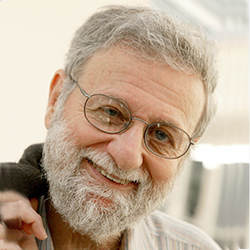
\includegraphics[width=4cm, height=4cm]{norman-don.jpg}
\centering
\end{figure}
\end{itemize}
\end{frame}

\section{Contributions}
%References frame
\begin{frame}
\frametitle{Contributions}
\begin{itemize}
\item Su mayor aporte en la rama de la computación podríamos hacer referencias a las publicaciones en cuanto a la usabilidad. 
\item  Según Donald Norman , hay dos principios claves para una buena interacción humano-computadora: Visibilidad y Provisión.
\item Apesar de que las pautas de diseño propuestas por varios investigadores señalan que estas deben ser aplicadas cuidadosamente por personas expertas en el arte de la interfaz de usuario, Donald las proporciona como listas simples de edictos de diseño con poca o ninguna relación.
\item Norman incluyó los errores cognitivos en las pautas de diseño porque buscaba que alguno de estos (diseños) redujera o eliminara el impacto de los errores, que son comunes en humanos. 
\end{itemize}
\end{frame}

%References frame
\begin{frame}
\frametitle{Contributions}
\begin{itemize}
\item Los términos "gulfs of execution" y "gulfs of evaluation" fueron introducidos y popularizados por Donald. El primero se refiere al abismo existente entre lo que quiere el usuario de una herramienta y las operaciones que la herramienta proporciona, y el segundo al grado en el que la herramienta proporciona información de su estado que pueden interpretarse y emplearse directamente por el usuario.
\item Las primeras pautas de diseño humano-computadora de Norman se basaron en la investigación, la suya y la de otros, sobre la cognición humana.

\end{itemize}
\end{frame}

%References frame
\begin{frame}
\frametitle{Contributions}

\textbf{Los cuatro principios del buen diseño de Donald Norman:}
En su libro “Psicología de los objetos cotidianos” norman analiza los errores de diseño mas comunes, las causas cognitivas que están tras ellos y propone unos principios de diseño que son una referencia para cualquiera que se dedique al diseño de interacción. El libro trata bastantes conceptos y principios, que se pueden resumir en cuatro:

\begin{enumerate}
    \item Visibilidad
    \item Buena topografía
    \item Retroalimentación
    \item Buen modelo conceptual
\end{enumerate}

\end{frame}
\begin{frame}{Contributions}
\textcolor{red}{Compensaciones}\textbf{(El diseño es una serie de compensaciones)}
\begin{itemize}
    \item Cualquier técnica de diseño individual puede tener sus virtudes en una dimensión compensadas por deficiencias en otra. \item Agregue ayuda adicional para el usuario no calificado y corre el riesgo de frustrar al usuario experimentado.
    \item Agranda la pantalla y algunas tareas mejoran, pero otras se vuelven más confusas. 
    \item Es bien sabido que las diferentes tareas y clases de usuarios tienen diferentes necesidades y requisitos.
    \item Muestra más información y aumenta el tiempo para pintar la pantalla, aumenta el requisito de memoria, los programas se vuelven más grandes, más voluminosos, más lentos. 
\end{itemize}
\end{frame}
\begin{frame}{Contributions}
\textcolor{red}{Prototipo TradeOff:}\textbf{ (Información vs tiempo)}
\begin{itemize}
    \item Por un lado, cuanto más informativa y completa es la pantalla, más útil cuando el usuario tiene dudas o falta de comprensión, 
    \item Por otra parte, cuanto más completa es la pantalla, más tiempo tarda en mostrarse y más espacio debe ocupar físicamente. \item Este es uno de los principales problemas de interfaz que deben manejarse
\end{itemize}
\end{frame}

\section{References}
%References frame
\begin{frame}
\frametitle{References}
\begin{itemize}
\item Intdrouction - xiii, Jhonson J. (2014). Designing with the Mind in mind. 2nd. edition.
\item Norman, D. A. (1998). La psicología de los objetos cotidianos (Vol. 6). Editorial Nerea.
\item Norman, D. A. (1986). Cognitive engineering. En: User centered system desing: New perspectives on human–computer interaction. Hillsdale, NJ: Erlbaum Associates.
\end{itemize}
\end{frame}

\end{document}